\documentclass[10pt,letterpaper]{article}
\usepackage[latin1]{inputenc}
\usepackage{indentfirst}
\usepackage{amsmath}
\usepackage{amsfonts}
\usepackage{amssymb}
\usepackage{hyperref}
\usepackage{listings}
\usepackage{pdflscape}
\usepackage{geometry}
\usepackage{array}

\usepackage{todonotes}

\DeclareMathOperator*{\argmax}{arg\!max}

\author{Andrew Price, advised by Frank Dellaert and Charlie Kemp}
\title{Planar Segmentation of Multiview RGB-D Image Sets using Markov Chain Monte Carlo }
\date{}

\begin{document}
\maketitle

\section{Abstract}
	As techniques for reconstructing 3D scenes have progressed beyond purely geometric modelling, attention has now shifted to techniques for understanding the content of these captured scenes. An important intermediate step towards this goal is to be able to segment different objects in the environment from one another, so that recognition can be performed on manageable and consistent components of the captured 3D world. With this objective in view, one possible first step is to begin by first segmenting the world into geometric primitives, in this case planes. This paper presents a method for applying the Swendsen-Wang Markov Chain Monte Carlo approach to simultaneously compute the optimal segmentation for a set of RGB-D images.
	
\section{Introduction}
	Any introduction to a discussion on modern 3D image segmentation or reconstruction ought to begin with an acknowledgement of the impact of consumer RGB-D cameras like the Microsoft Kinect and its brethren from Asus and PrimeSense. Following the Kinect's release in late 2010, there has been an explosion of academic, commercial, and hobbyist applications for the relatively inexpensive devices, spanning such diverse topics as simultaneous localization and mapping, additive manufacturing, visual servoing, and the original purpose of novel user interfaces. Thus, the benefits of developing and extending algorithms that operate on these types of RGB-D data must be readily apparent to the reader.
	
	Much of this research has focused on methods of reconstructing an environment geometrically, first using sparse, point-based methods (\cite{henry2010rgb}), then moving more towards volumetric dense methods. Many recent advances in the real-time integration of RGB-D images, such as KinectFusion (\cite{newcombe2011kinectfusion}) or Kintinuous (\cite{whelan2012kintinuous}) have leveraged modern general-purpose graphical processors (GPGPUs). While there are still a number of exciting challenges in the realm of geometric reconstruction, we will look ahead to the work of understanding content within a scene, beginning with image segmentation.
	
\section{Related Work}
	Myriad approaches have been proposed for the 3D image segmentation problem, including RANSAC-based model fitting, region growing, difference of normals, and graph cut methods, with many variations and combinations of these themes. For a general overview of segmentation methods applied to LIDAR captures, the reader is referred to \cite{douillard2011segmentation}. 
	
	For the similar problem of segmenting point clouds derived from colored stereo images, graph cuts have been shown to be effective for segmentation(\cite{bleyer2005graph}).

	
	We wish to strike out in a somewhat different direction from the main branch of research in this area in a couple of different ways. First, we wish to avoid becoming trapped in a local convergence basin, a common limitation of greedy segmentation algorithms. To accomplish this, we employ a modified version of the Markov chain Monte Carlo method described by Swendsen and Wang in 1987 (\cite{swendsen1987nonuniversal}), generalized to arbitrary probability densities by Barbu and Zhu in \cite{barbu2005generalizing}, and applied to RGB-D images by Erdogan, Paluri, and Dellaert in \cite{Erdogan12crv}. Such MCMC methods have proven relatively popular for reconstructing surfaces, as shown in \cite{tu2002image}, \cite{qiu2009jump}, and 	\cite{dick2002bayesian}.
	
	Second we choose to perform the segmentation simultaneously on the individual images, rather than fusing all of the images into a single point cloud or volume model. This allows the sampling algorithm to operate directly on the data as it was captured, rather than operating on an aggregated or fused model generated from many separate images.

\section{Procedure}

\subsection{Problem Definition: Graph Partitioning}

	Before moving on to the specifics of the multiview RGB-D segmentation, we begin by clarifying the more general graph partitioning problem. We define a graph $G<V,E>$ containing vertices $V=\{v_1,v_2,\ldots,v_M\}$ and edges $E$, where each vertex $v_j$ represents an atomic region in an image, or "superpixel". We now wish to find a partition $\pi_n=(V_1,V_2,\ldots,V_n)$ that correctly assigns atomic regions  $v_{j_s}\in{V_j}$. A partition is an assignment of each edge $e_{s,t}$ in graph $G$ to either "on" or "off". An atomic region must exist uniquely in a segment, that is, $\bigcup_{i=1}^{n}V_i=V$ and $V_i\bigcap{V_j}=\emptyset,\forall{i}\neq{j}$.
	
	Additionally, we wish to fit a parameterized model to each segment $V_i$. The full model assigned consists of a model family $l\in{L}$,  $L=$\{planar, cylindrical, spherical, spline, etc.\}, that describes the nature of the underlying surface, as well as a parameterization $\theta_i$ $i=1,2,\ldots,n$ containing the coefficients for the given model type. For the plane model (used exclusively in this paper), these are the coefficients from the plane equation $ax+by+cz=d$. We can combine these components into a full model description $c_i=(l_i,\theta_i)$ $i=1,2,\ldots,n$ that is analogous to the graph color assignment in \cite{swendsen1987nonuniversal}.
	
	Armed with descriptions of both which superpixels are associated with one another and what model describes these segments, we can construct a full world description $W=(n,\pi_n,c_1,c_2,\ldots,c_n)$. The  This is the function we are trying to optimize via $W^*={\argmax}_{W\in\Omega} P(I|W)P(W)$. For our problem, the search space $\Omega$ is very large, with $\Omega=\bigcup_{n=1}^{|V|}\{\Omega_{\pi_n} \times\Omega_{l}^n \times\Omega_{\theta_1} \times\Omega_{\theta_2},\ldots, \times\Omega_{\theta_n}\}$.


\subsection{Image Graph Generation}
	In order to generate an initial oversegmentation and adjacency graph for each image in the set, we adhere closely to the work presented in \cite{Erdogan12crv}. We employ a modified version of the Felzenszwalb-Huttenlocher graph-cut algorithm presented in \cite{felzenszwalb2004efficient}, adding factors for both color and depth components in the image.
\begin{equation}
w_{i,j}=\alpha w_C + \beta w_D + \gamma w_S
\end{equation}
\begin{align*}
w_C&=\sqrt{(r_i-r_j)^2+(g_i-g_j)^2+(b_i-b_j)^2+(z_i-z_j)^2} \\
w_D&=abs(z_i-z_j) \\
w_S&=\sqrt{(u_i-u_j)^2+(v_i-v_j)^2} \\
\end{align*}
	Next, we compute a set of properties, $\rho$, for each superpixel. These properties will help us to generate more efficient proposal densities when we wish to sample from the graph configurations. We achieve this by incorporating a discriminative probability $q_e$ for each edge $e\in{E}$ determined by the following equation:
\begin{equation}
	q_e=P(\mu_e=on|\rho_s,\rho_t)=e^{\|w_\rho\odot(\rho_s-\rho_t)\|^2\frac{T}{2}}
	\label{eq:edgeProb}
\end{equation}
where $\mu_e$ is a random binary variable following a Bernoulli distribution and representing the state of an edge in a given sample, $w_\rho$ is a weight vector to account for the various units used (neighboring pixel distances might be on the order of 0.01m, while color differences might be on the order of 10 units), $\odot$ represents element-wise vector multiplication, and $T$ is a temperature factor. In this implementation, $\rho$ is composed of the plane parameters and centroid for each superpixel, but color or normal histograms have also been used.

\subsection{World Graph Generation}
	Having generated a weighted superpixel adjacency graph for each image $I_t$ in the input sequence, we now wish to create a world graph $G'_t$ incorporating each individual image graph $G_t$ as a subgraph. $G'$ contains all vertices representing the superpixels, i.e.,
\begin{equation}
	V'_t=V'_{t-1}{\bigcup}V_t
\end{equation}
	 Additionally, this global graph contains all original edges, plus edges that we will add to relate the individual frames to each other,
\begin{eqnarray}
	 E'_t=E'_{t-1}{\bigcup}E_t{\bigcup}E(\rho'_s,\rho_k) \\
s=1,2,\ldots,\sum_{\tau=1}^{t-1}{N_\tau}\nonumber \\
K=1,2,\ldots,N_t\nonumber
\end{eqnarray}	 
	The edge generating function $E(\rho'_s,\rho_k)$ is a thresholded version of equation \ref{eq:edgeProb}, where edges are only added if $q_e>q_0$, where $q_0$ is some experimentally determined threshold value.
	
%	 The adjacency graph for the image at time $t$
% The world graph incorporating all images up to time $t$
% Set of vertices at time $t$

\subsection{World Graph Sampling}
	An initial partition $\pi_0$ is achieved by turning off edges in the graph according to edge weights $q_e$. The connected components following this operation are the initial segments $\{V_1,V_2,\ldots,V_n\}$. For each of these segments, we compute a best fit surface with parameters $\theta$. The probability of the full segmentation is
\begin{equation}
P(\pi|Z) \propto P(\pi)\prod_{V_j\in \pi}e^{- Err(\theta_{j}^*, V_j,Z_j)/2}\sqrt{|2\pi\Sigma_j|}
\end{equation}
where $Err(\theta_{j}^*, V_j,Z_j)$ represents the error between the data and the best fit parameters, and $\sqrt{|2\pi\Sigma_j|}$ is an information term to avoid over-fitting.

	We wish to now sample this graph-based configuration space in proportion to the posterior probability density. As shown in the Metropolis-Hastings algorithm (\cite{metropolis1953equation}), this can be achieved even with an unknown posterior function by introducing an acceptance ratio $a$ for a new proposed state as $a=\frac{P(x')}{P(x_t)}$, where $x'$ is a proposed state and $x_t$ is the current state. Proposed states producing $a\geq 1$ are accepted automatically, while others are accepted with probability $a$.
	
	The discriminative probabilities $q_e$ on each edge form the basis for the proposal density for generating new $x'$s. Algorithmically, this is implemented by randomly selecting a superpixel and recursively growing the region probabilistically according to the edge weights. We will call this connected component $C^*$, and propose to either flip it to an adjacent segment, or to split it into its own segment. More concisely, we will propose to flip $C^*$ as follows: 
\begin{equation}
C^*\subset V_a \in \pi^A \Rightarrow C^*\subset V_b \in \pi^B
\end{equation}
	
	Conveniently, since we are only proposing to change the configuration of two segments, $V_a$ and $V_b$, the acceptance ratio $a(\pi^{A}\rightarrow \pi^{B})$ only depends on $V_a$ and $V_b$, so we avoid the overhead of having to compute the probability of the full segmentation $\pi^B$:

\begin{equation}
a(\pi^{A}\rightarrow \pi^{B})=\frac{\prod_{e\in E(C^{*},V_{a}-C^{*})}(1-q_{e})\, q(V_{a}|C^{*},\pi^{B})\, p(\pi^{B}|Z)}{\prod_{e\in E(C^{*},V_{b}-C^{*})}(1-q_{e})\, q(V_{b}|C^{*},\pi^{A})\, p(\pi^{A}|Z)}\label{eq: acceptanceRatio}
\end{equation}

\begin{eqnarray}
\frac{p(\pi^{B}|Z)}{p(\pi^{A}|Z)} & = & \frac{P(\pi^{B})\prod_{V_{i}\in \pi^{B}}P(V_{i}|Z_{i})}{P(\pi^{A})\prod_{V_{j}\in \pi^{A}}P(V_{j}|Z_{j})}\nonumber \\
 & = & \frac{P(V_{a}^{B}|Z)P(V_{b}^{B}|Z)}{P(V_{a}^{A}|Z)P(V_{b}^{A}|Z)}\label{eq:jumpProb}
\end{eqnarray}

	Equipped with this acceptance ratio, we can now proceed to sample from the world graph by performing the following: creating an initial random partition, selecting a (possibly weighted) random superpixel, collecting some of its neighbors in a Swendsen-Wang cut, proposing to move this connected component to a new segment $V_b$, and accepting the move according to our acceptance equation.


%	$I_t$ RGB-D Image at time $t$ This represents the stream of images to be segmented
%
%$q_e=P(\mu_e=on|c_i,c_j)$ $e\in{E}$ Discriminative probability on edge $e$. $\mu_e$ is a binary random variable following a Bernoulli distribution and describing the probability of two adjacent vertices in $G'_0(t)$ being connected in a given step.
%$E'_t(\pi)\subset{E'_t}$ Set of edges turned on for partition $\pi$ at time $t$

\section{Results}
	In order to test the effectiveness of the proposed method, we ran the algorithm on datasets provided by \cite{sturm12iros}. ROS (\cite{ros2009}) provided the data communication and visualization capabilities, and OpenCV (\cite{opencv_library}) and PCL (\cite{rusu20113d}) provided many of the utilities for operating on the images and point clouds, respectively. Unfortunately, the complete solution has not been fully implemented as of the time of writing, but the current status of results may still be discussed.

\begin{figure}[ht]
\begin{center}
	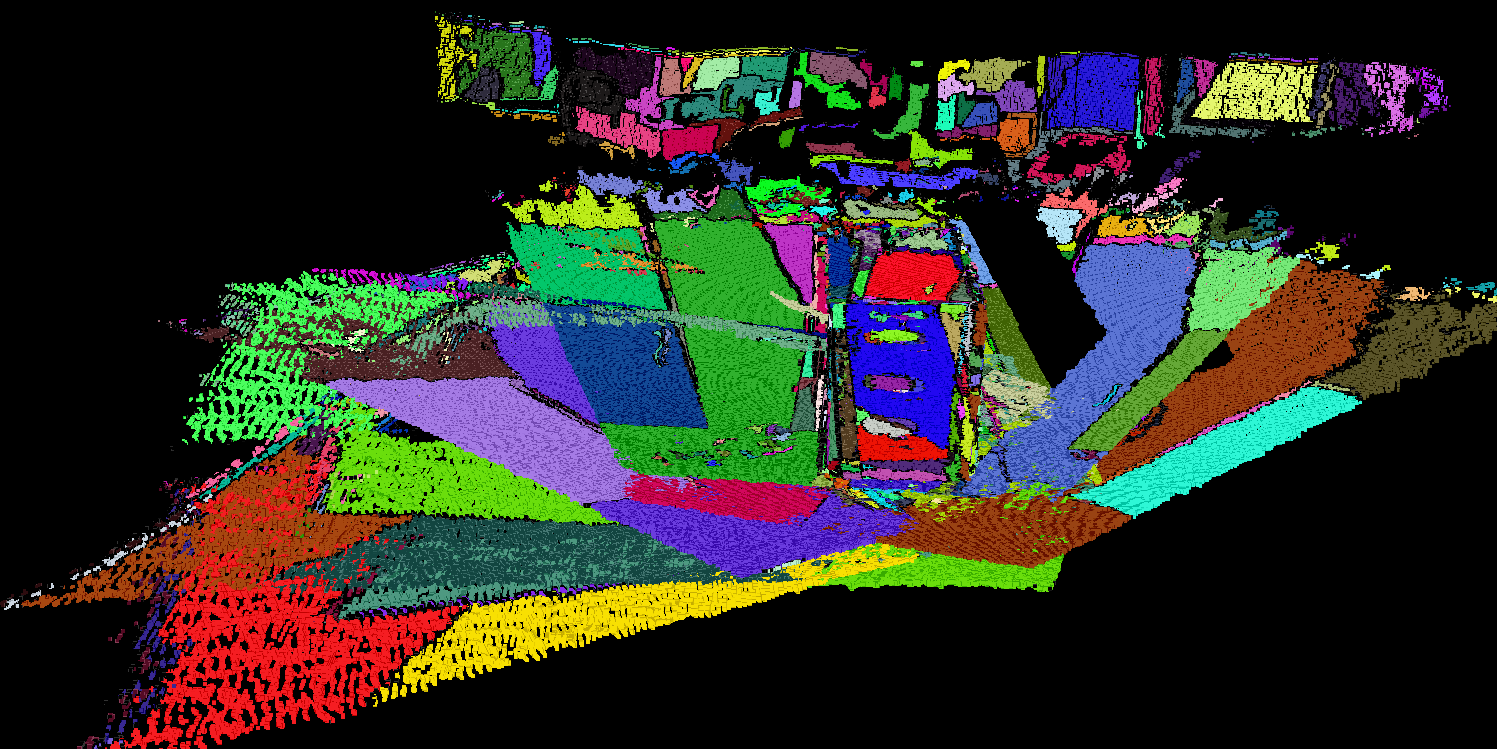
\includegraphics[width=.9\linewidth]{OverSegmented1.png}
\end{center}
\caption{Oversegmented RGB-D images projected into 3D scene.}
\label{fig:overseg1}
\end{figure}

\begin{figure}[ht]
\begin{center}
	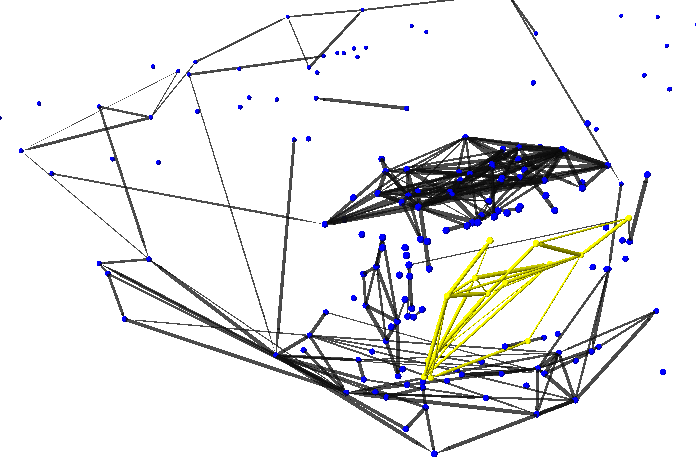
\includegraphics[width=.9\linewidth]{graph1.png}
\end{center}
\caption{3D adjacency graph with one S-W cut highlighted.}
\label{fig:highGraph}
\end{figure}

	Figures \ref{fig:overseg1}, \ref{fig:overseg2}, and \ref{fig:overseg3} show the results of the oversegmentation algorithm when applied over several RGB-D images in a sequence and projected into a consistent 3D frame. Figure \ref{fig:highGraph} shows a sample world graph created from the individual images' superpixels. In the figure, one can observe the highly connected nature of the sets of regions that correspond to the same underlying surfaces. While this is the desired behavior, it is actually something of a mixed blessing, as we will explore in the next section.

\section{Conclusions}
\subsection{Strengths}
	The techniques presented here appear to be a strong initial attempt at generating a simultaneous segmentation for registered RGB-D images. The values selected for generating the discriminative probabilities, $\rho$ and $q_e$, generate graphs that are strongly connected to other nodes within the same plane, and weakly coupled to other parts of the environment. The full implementation must be completed before a final assessment of the accuracy of the segmentation can be carried out, however.
\subsection{Potential Improvements}

	Perhaps the most direct potential improvement would be to optimize the camera poses with respect to the computed segmentation. Currently, the results shown use the recorded ground truth positions for the camera extrinsic parameters. In a more realistic scenario, this information is unlikely to be provided, so correctly matching surface models would provide a potential way to inform a pose-graph optimization using something like GTSAM (\cite{gtsam}).
	
	One of the more significant challenges to address going forward is the issue of overconnected components. For example, imagine a segment that contains $n$ superpixels: $V_1=\{v_1,v_2,\ldots,v_n\}$. If there are strong correspondences between the best fit planes for the segments, which there ought to be if the data truly does correspond to the same underlying surface, then the subgraph of $V_1$ will be very densely connected, perhaps even a complete graph. For this situation, even with relatively low probabilities on each edge, there is a strong chance that the recursive growth algorithm will still select the entire segment, as each node has $\approx n$ chances to be selected into the connected component. One proposed method to combat this issue would be to create a maximum probability spanning tree starting with the selected root superpixel. This would mean that each node is only added to the component with a probability equal to the most likely path, rather than the cumulative probability of all of the possible paths.

\bibliography{references}
\bibliographystyle{unsrt}

\begin{figure}[ht]
\begin{center}
	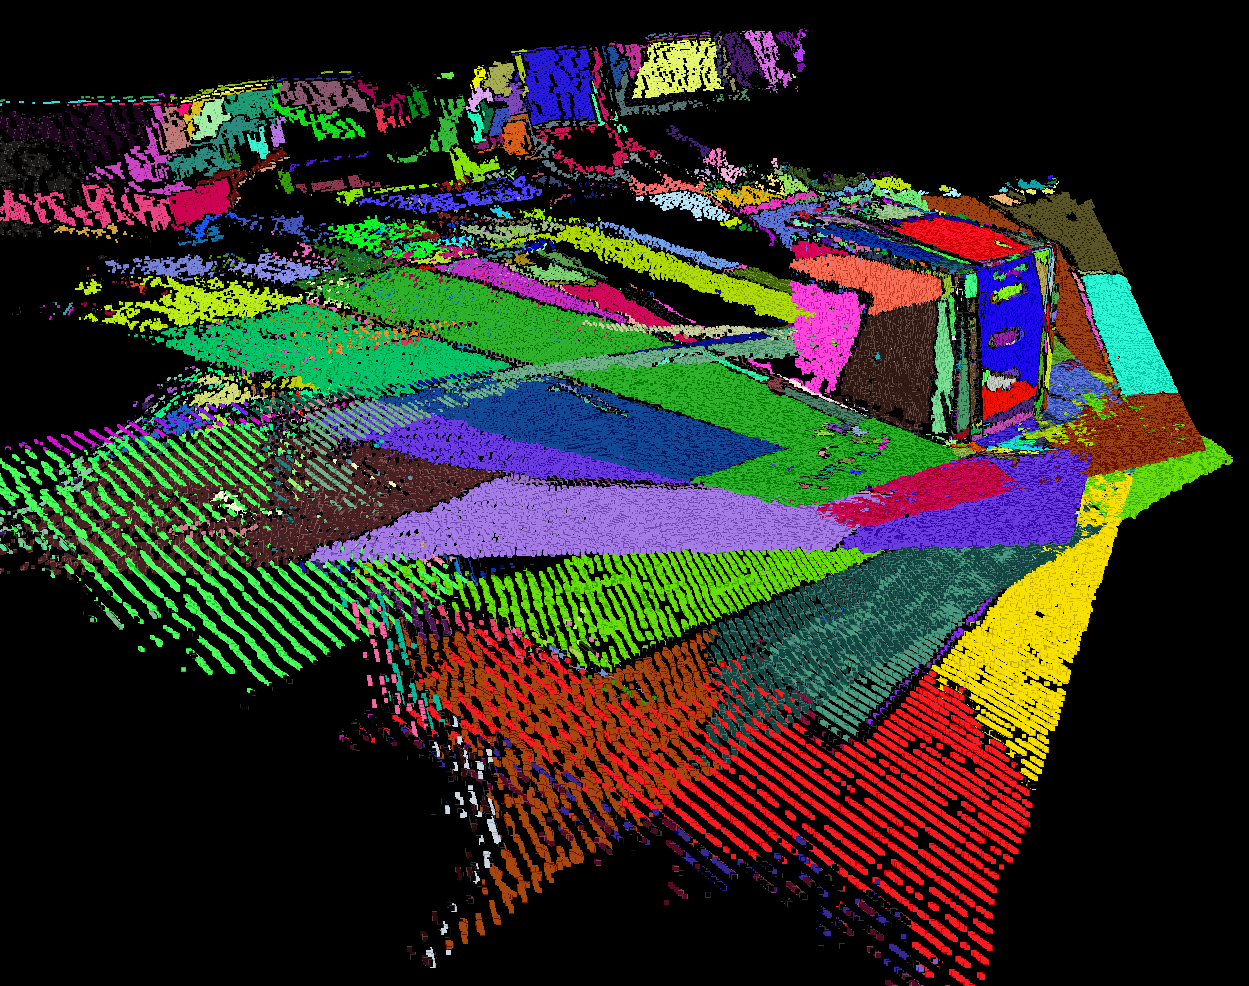
\includegraphics[width=.4\linewidth]{OverSegmented2.png}
\end{center}
\caption{Oversegmented RGB-D images projected into 3D scene.}
\label{fig:overseg2}
\end{figure}

\begin{figure}[ht]
\begin{center}
	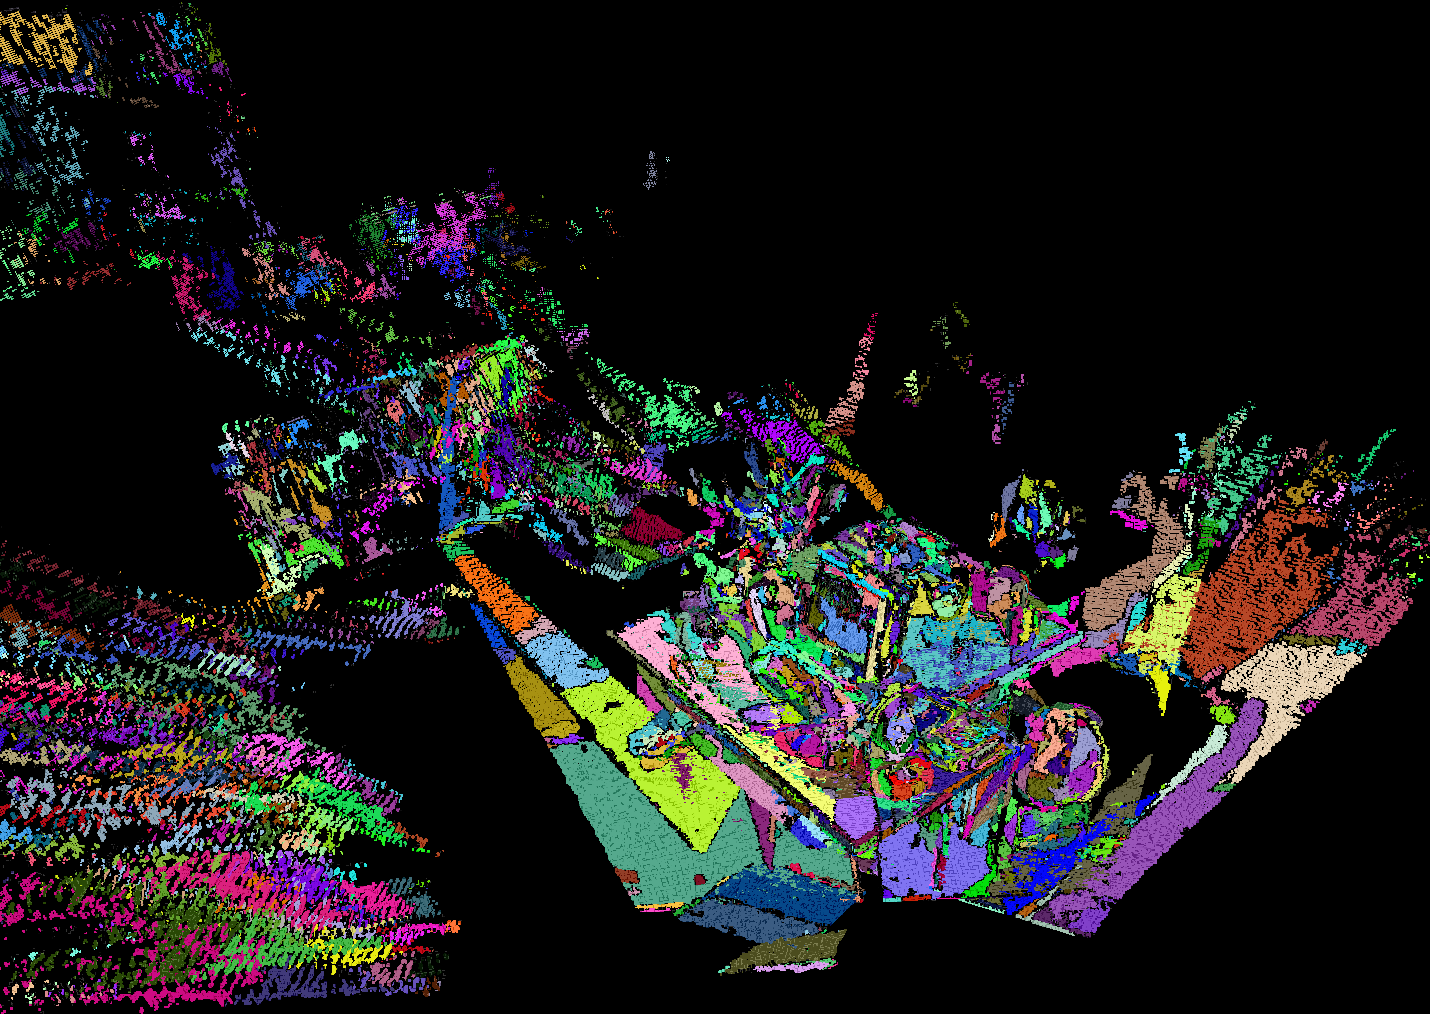
\includegraphics[width=.4\linewidth]{OverSegmented3.png}
\end{center}
\caption{Oversegmented RGB-D images projected into 3D scene.}
\label{fig:overseg3}
\end{figure}

\end{document}